\section{Data Import}
\label{sec:dataimport}
There are several ways to import data into Germinate. Some people may prefer to write their own scripts to import the data whereas others may prefer database management tools like \textit{Navicat} \cite{Navicat}, \textit{MySQL Workbench} \cite{MySQLWorkbench} etc.

However, we believe that we can make the import process even easier and so we developed a Java based desktop application to aid in the upload of experimental datasets into Germinate. The aim of this tool is to simplify the process of entering data into the system. \textit{Germinate 3 Data Importer} (G3DI) allows permitted MySQL system users to upload data in text file format into a specified Germinate installation. We have also included tools to revert the most recent change should any problems arise in the data upload process.\\
\\
The Germinate 3 Data Importer can be downloaded here:

\begin{center}
    \url{http://ics.hutton.ac.uk/g3di/}
\end{center}

\begin{figure}
    \centering
    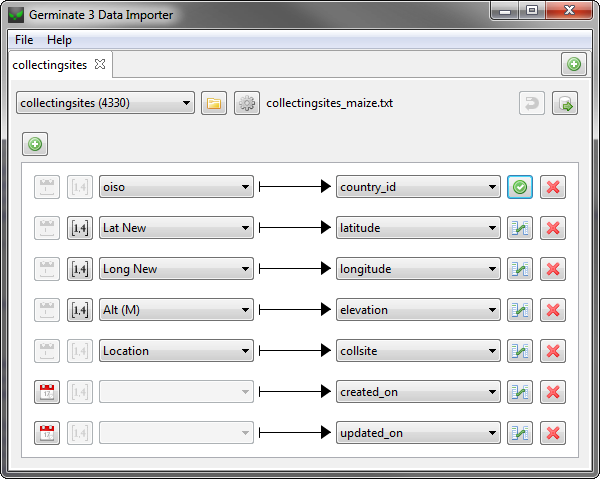
\includegraphics[scale=0.6]{img/import/g3di-mapping.png}
    \caption{G3DI - Column mapping}
    \label{fig:g3di-mapping}
\end{figure}

\noindent Figure \ref{fig:g3di-mapping} shows the main GUI of G3DI with an example mapping. The current tab is used to import data from a text file with the name \texttt{collectingsites\textunderscore maize.txt} into the database table \texttt{collectingsites}. Each row represents a mapping between column of the input file and column of the database. G3DI is aware of the data types of the database columns and provides functionality to accommodate dates, number formats and foreign keys. The first row of the mapping maps \texttt{oiso} (which is a 3-digit country code) to \texttt{country\textunderscore id}. G3DI knows that \texttt{country\textunderscore id} is a foreign key column and requests the user to define a lookup table and column. This lookup is used to find the foreign id based on the value in the \texttt{oiso} column.

As an example, let's assume the lookup table is \texttt{countries} and the lookup column is \texttt{country\textunderscore code3} and the value in the column \texttt{oiso} is "GBR". G3DI will then query the database and determine the id of the country with the 3-digit code "GBR" (which is the United Kingdom) and use this id instead of the actual value.

In addition you can define a number format (or to be exact, a locale) for decimal columns. This format is used to parse your input data before inserting it into the database.

Finally, you can define date formats for columns that represent dates. As an example, let's say your input data is in the form \texttt{dd/MM/yyyy} (2-digit day, 2-digit month, 4-digit year). G3DI will then parse your dates before inserting them into the database. This is necessary, since the database uses its own date format which may differ from the format you used for your data.\\
\\
After you imported your data, you might realize that your mapping was incorrect. G3DI can undo the most recent import step with one click of a button, to allow you to do your work without worrying that you might mess up the database. If you want to be on the safe side, you can still make a backup of the whole database with your favourite database management tool.